\documentclass{beamer}
\usepackage{hyperref}
\usepackage{colortbl}
\usepackage{fourier}
\usepackage[T1]{fontenc}

% other packages
\usepackage{latexsym,amsmath,xcolor,multicol,booktabs,calligra}
\usepackage{graphicx,listings,stackengine}
\usepackage{subcaption}
\usepackage{xcolor}
\usepackage{tabularx}
\usepackage{tikz}
\renewcommand\tabularxcolumn[1]{m{#1}}  % vertical centering of text in tabularx 
\newcommand\Mark[2][8.4]{%
	\rlap{\tikz[baseline=(current bounding box.south)]{
			\shade[left color=red, right color=green!#2!red]
			(0,0) rectangle ++(#1*#2/100,0.3);}%
	}%
}

\definecolor{vtxtablegray}{RGB}{208, 213, 215}

\DeclareCaptionFormat{myformat}{\textbf{#1#2}#3}
 \captionsetup{format=myformat}

% \author{Gerard Castro}

\title{Interpretable Convolutional Neural Networks}
\subtitle{Quanshi Zhang, Ying Nian Wu \& Song-Chun Zhu (UCLA)}
\institute{% 
\includegraphics[width=0.025\linewidth]{img/ub.png}\vspace{5mm}\  
Universitat de Barcelona}
\author{Gerard Castro}
\date{\today}
\usepackage{style}


% defs
\def\cmd#1{\texttt{\color{red}\footnotesize $\backslash$#1}}
\def\env#1{\texttt{\color{blue}\footnotesize #1}}
\definecolor{deepblue}{rgb}{0,0,0.5}
\definecolor{deepred}{rgb}{0.6,0,0}
\definecolor{deepgreen}{rgb}{0,0.5,0}
\definecolor{halfgray}{gray}{0.55}

\newcommand\checkitem{\item[\color{green}\checkmark]}
\newcommand\dangeritem{\item[\color{yellow}\danger]}
\newcommand\crossitem{\item[\color{red}\texttimes]}

\lstset{
    basicstyle=\ttfamily\small,
    keywordstyle=\bfseries\color{deepblue},
    emphstyle=\ttfamily\color{deepred},    % Custom highlighting style
    stringstyle=\color{deepgreen},
    numbers=left,
    numberstyle=\small\color{halfgray},
    rulesepcolor=\color{red!20!green!20!blue!20},
    frame=shadowbox,
}


\begin{document}

\begin{frame}
    \titlepage
    \begin{figure}[htpb]
        \begin{center}
           
\includegraphics[width=0.4\linewidth]{img/fmiub.png}
        \end{center}
    \end{figure}
\end{frame}


\section{Introduction}

\begin{frame}{Idea}
    This paper proposes a CNN \textbf{design} for object \textbf{classification} which is more \textbf{interpretable} by construction.
    \begin{itemize}[<+->]  
        \item \textbf{What does this mean?} 
        \item  That feature map activations (in high \textbf{convolutional layers}) just \textbf{focus} on a \textbf{single} object \textbf{part}
        % By introducing a local loss term \textbf{for each} \textbf{filter} in these conv. layers such that encourages the filter to be activated by a \textbf{single object part}. % (rather than repetitively appear on different object regions).
        % \textbf{regularize} the representations ensuring the interpretability
        % \item The method does \textbf{not need different} training \textbf{data} or additional types of annotations, but the custom loss encourages the filter to be activated by a single part of the object (rather than repetitively appear on different object regions).  
    \end{itemize}
\end{frame}

\begin{frame}{Motivation}
	Interpretability is as \textbf{crucial} as discriminative power, necessary both to:
	\begin{itemize}[<+->]
        \item  \textbf{Understand} a network to be able \textbf{to keep improving} it
        \item \textbf{Trust} the network by \textbf{explaining its logic} for decisions % (\textit{i.e.} what patterns are memorized and used for prediction). Besides, whereas there are many ways to asses interpretability (\textit{gradient-based attribution, network dissection, ablation studies}...); but this is one of the few techniques which proposes interpretability as an end-to-end \textit{learning task}
    \end{itemize}
\end{frame}

\section{Technical description}

\begin{frame}{\textit{Regularizing} the interpretability}
    Let x be a feature map % \footnote{Note a feature map is simply applying the filter $f$ to an input image $I$, $x := f(I)$.}
    ($n\times n$) for a filter $f$ in the top conv. layers; and $c$ a object category.\vspace{2mm}
    
	\textbf{Key idea}: to \textbf{push} each filter $f$ to \textbf{focus} on a \textbf{single} object part $\textbf{c}$. % 
    \textbf{How?}
	\begin{itemize}[<+->]
        \item In the \textbf{forward propagation} (applying filters):
        \begin{itemize}[<+->]
            \item Applying a L1 or L2 mask to the feature map $x$ obtaining $x^{\mathrm{masked}}$ 
        \end{itemize}
        \item In the \textbf{backward propagation} (learning filters):
        \begin{itemize}[<+->]
            \item \textbf{Assigning} a \textbf{category} $c$ to each filter $f$
            \begin{itemize}
                \item The assigned category $c^{*}$ is that which activates $f$ most: $c^{*}:=\mathrm{argmax}_c\ \mathrm{mean}_{x\in I_c \subset I }\ \sum_{i, j}x_{ij}$
            \end{itemize}
            \item \textbf{Adding} a \textbf{loss term} $\mathbf{\mathrm{Loss}}_f$ for each filter (depends on the assigned $c$)
            \begin{itemize}
                \item This loss term $\mathbf{\mathrm{Loss}}_f$ will \textbf{regularize} the filter activation to ensure it \textbf{just focuses on} the category $\textbf{c}$
            \end{itemize}
        \end{itemize}
    \end{itemize}
    
\end{frame}

% FILTERS figure

% \begin{frame}{Forward propagation}
% 	During \textbf{forward propagation}: we will obtain the \textbf{masked} version $x^{\mathrm{masked}}$ of $x$ by:
% 	\begin{itemize}[<+->]
        % \item Defining a template of $n^2$ masks for the feature map $x$: $\{T_{\mu_1}, \ldots, T_{\mu_{n^2}}\}$
    % \end{itemize}
    % \begin{figure}
        % \centering
        % 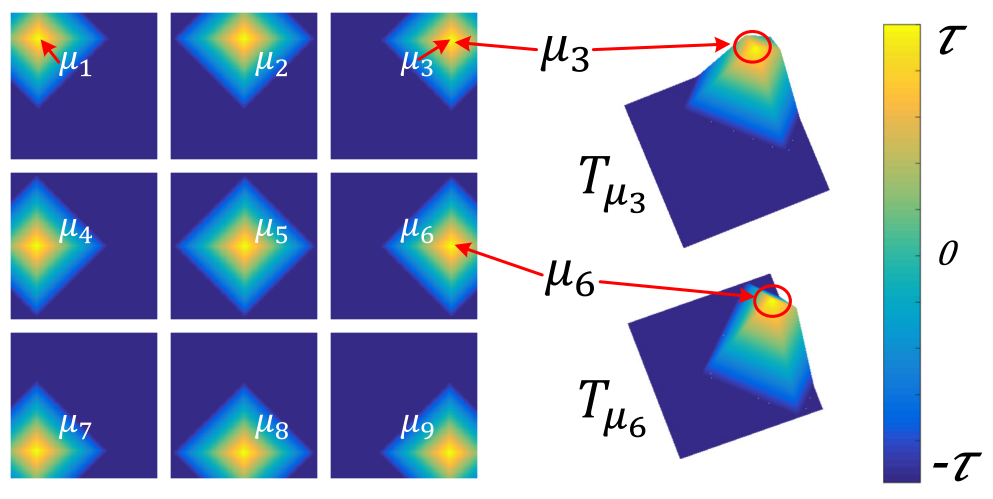
\includegraphics[width=0.6\linewidth]{figures/filters.png}
        % \caption{Templates of $T_{\mu_i}$ masks based on the L-1 norm}
    %     \label{fig:mask_templates}
    % \end{figure}
% \end{frame}

% EXPLANATION of x^masked (forward propagation)

\begin{frame}{Forward propagation}
	During \textbf{forward propagation}: we obtain the \textbf{masked} version $x^{\mathrm{masked}}$ of $x$ by:
	\begin{itemize}[<+->]
        \item Defining a template of $n^2$ masks for $x$: $\{T_{\mu_1}, \ldots, T_{\mu_{n^2}}\}$
        \item Selecting the mask $T_{\mu^{*}}$ located in the highest activation region of $x$: $\mu^{*}= \mathrm{argmax}_{ [i, j]}x_{ij}$
        \item Applying the selected mask $T_{\mu^{*}}$ using $\circ$ Hadamard distance: $x^{\mathrm{masked}} := \max \{ x\circ T_{\mu^{*}}, 0 \}$
        % \item \textbf{Note}: different input images $I$ (thus, $x$) will have different masks $T_{\mu^{*}}$, in function of where the higher activation $(i, j)$ is
    \end{itemize}
\end{frame}

% Figure of the chosen mask

\begin{frame}{Forward propagation}
	During \textbf{forward propagation}: we will obtain the \textbf{masked} version $x^{\mathrm{masked}}$ of $x$ by:
    \begin{figure}
        \centering
        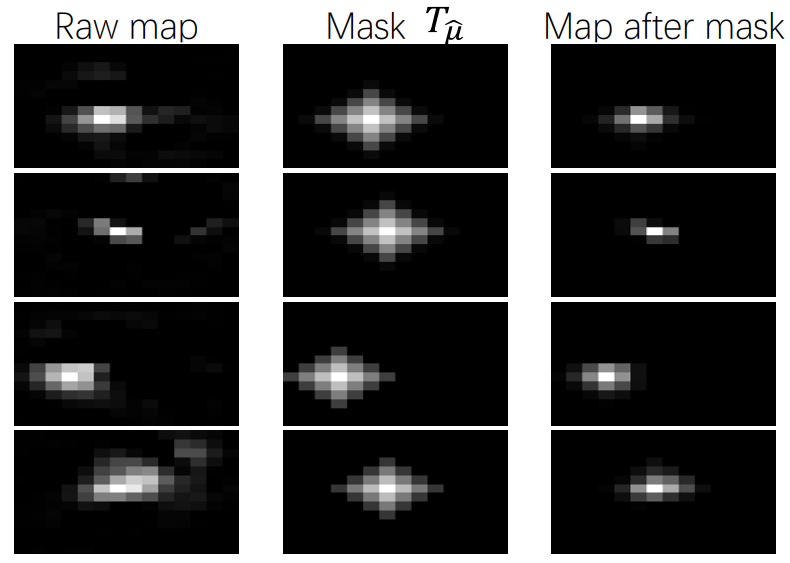
\includegraphics[width=0.65\linewidth]{figures/masks.png}
        \caption{Raw feature map $x$ (left), chosen mask $T_{\mu^{*}}$ (center) and map after mask $x^{\mathrm{masked}}$}
        \label{fig:chosen_mask}
    \end{figure}
\end{frame}

% LEARNING process (backwrd propagation)

% \begin{frame}{Backward propagation}
%     During \textbf{backward propagation}: for the filter $f$, the new loss term $\mathbf{\mathrm{Loss}}_f$ is added so that it \textbf{pushes the filter} to produce feature maps just \textbf{focused} on the assigned category $c^{*}$ for $f$ % (\textit{i.e.} $\mathbf{\mathrm{Loss}}_f$ depends on $c^{*}$) 
% 	\begin{itemize}[<+->]
%         \item The loss term is defined in terms of the \textbf{mutual information} between the feature maps $\textbf{X}$ and the mask templates $\textbf{T}$  
%         \item \textbf{And how the category is chosen?}
%         \item The filter $f$ is assigned with the category $c^{*}$ which activates $f$ most: $c^{*}:=\mathrm{argmax}_c\ \mathrm{mean}_{x\in I_c \subset I }\ \sum_{i, j}x_{ij}$
%     \end{itemize}
% \end{frame}

% LEARNING process (scheme FIGURE)

\begin{frame}{Backward propagation}
	During \textbf{backward propagation}: each filter $f$ receives gradients (\textit{w.r.t.} a feature map $x$) both from the final task loss $\mathbf{\mathrm{L}}(y_k^{*}, y_k)$ but also the \textbf{added} filter \textbf{loss term} $\mathbf{\mathrm{Loss}}_f$: $$ \frac{\partial \mathbf{\mathrm{Loss}}}{\partial x_{ij}} = \lambda\frac{\partial \mathbf{\mathrm{Loss}}_f}{\partial x_{ij}} + \frac{1}{N}\sum^{N}_{k} \frac{\partial \mathbf{\mathrm{L}}(y_k^{*}, y_k)}{\partial x_{ij}} $$ %; where $\lambda$ is a weight and $N$ the batch size.
    \begin{figure}
        \centering
        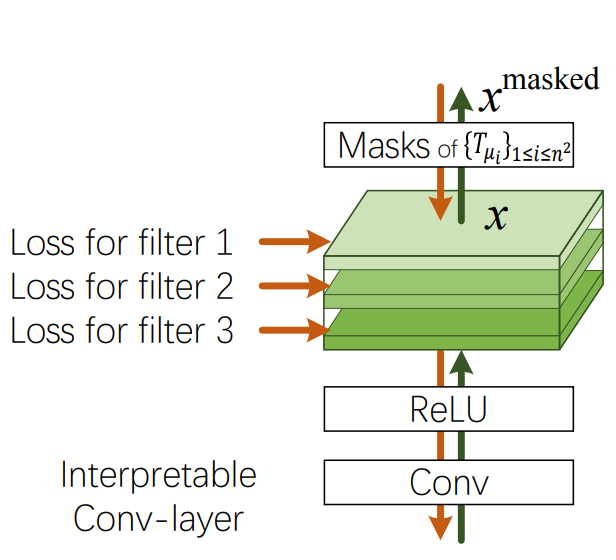
\includegraphics[width=0.35\linewidth]{figures/interpretable_cnn.png}
        \caption{The green (red) line indicates forward (backward) propagation}
        \label{fig:learning_scheme}
    \end{figure}
\end{frame}

\section{Results \& conclusions}

\begin{frame}{Benchmarks}
The authors used:
\begin{itemize}%[<+->]
    \item \textbf{3} benchmark \textbf{datasets} with landmark/part \textbf{annotations}: \textbf{37} animal \textbf{categories} defined
    \item \textbf{4} pre-trained CNNs (\textbf{AlexNet}, \textbf{VGG-M}, \textbf{VGG-S} \& \textbf{VGG-16}) \textbf{fine-tuned} with \textbf{interpretable} conv. \textbf{filters}
    \item \textbf{2} metrics to \textbf{assess} the clarity of the part \textbf{semantics} of a conv. filter: \textit{object-part interpretability}\footnote{Proposed by D. Bau, B. Zhou, A. Khosla, A. Oliva, and A. Torralba. \textbf{Network dissection: Quantifying interpretability of deep visual representations}. In \textit{CVPR}, 2017.} \& \textit{location stability}\footnote{Proposed by Q. Zhang, R. Cao, F. Shi, Y. Wu, and S.-C. Zhu. \textbf{Interpreting CNN knowledge using an explanatory graph}. In \textit{arXiv} 1708.01785, 2017.}
    \begin{itemize}[<+->]
        \item In \textbf{both metrics} (for all datasets \& architectures), the results sought with \textbf{interpretable CNN} were \textbf{superior}.
    \end{itemize}
\end{itemize}
\end{frame}

\begin{frame}{Results}
    \begin{figure}
        \centering
        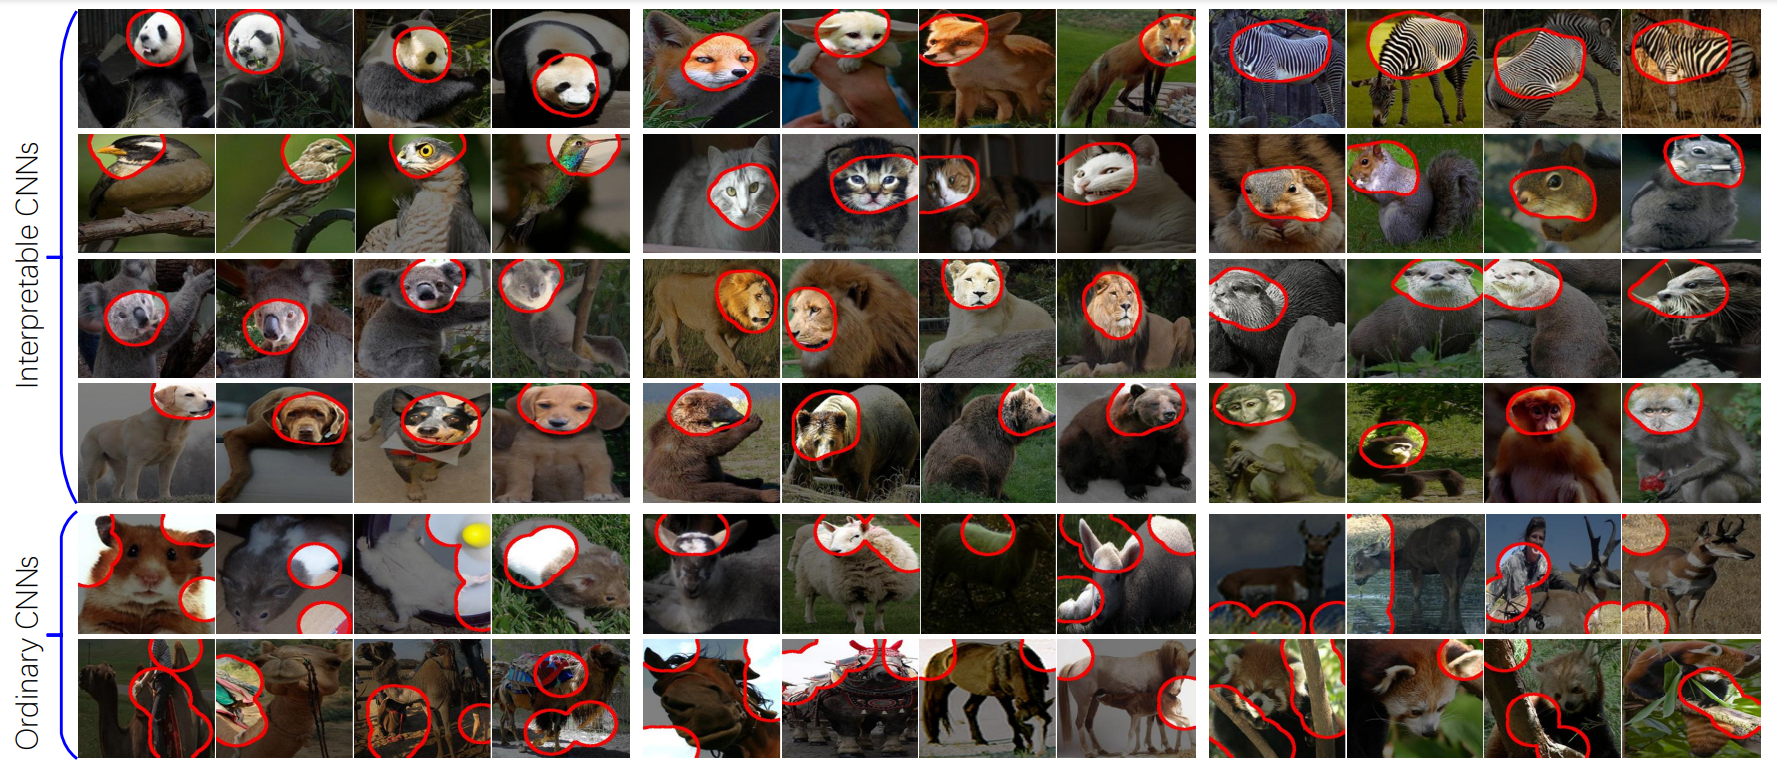
\includegraphics[width=1.00\linewidth]{figures/results.png}
        \caption{Visualization of filters in top conv. layers: for an interpretable (conventional) CNN in the 4 top rows (2 bottom rows). The receptive field of activations in a feature map were estimated according to \footnote{B. Zhou, A. Khosla, A. Lapedriza, A. Oliva, and A. Torralba. \textbf{Object detectors emerge in deep scene CNNs}. In \textit{ICRL}, 2015.}.}
        \label{fig:results}
    \end{figure}
\end{frame}

\begin{frame}{Conclusions}
    The authors conclude:
    \begin{itemize}[<+->]
        \item Their interpretable CNN \textbf{encoded} more \textbf{semantically} meaningful \textbf{knowledge} in high conv. layers than traditional CNN
        \item Despite a potential \textbf{trade-off} between \textbf{interpretability} and \textbf{discriminative power}, \textbf{better} results were \textbf{achieved} in \textbf{multi-category} classification:
        \begin{figure}
        \centering
        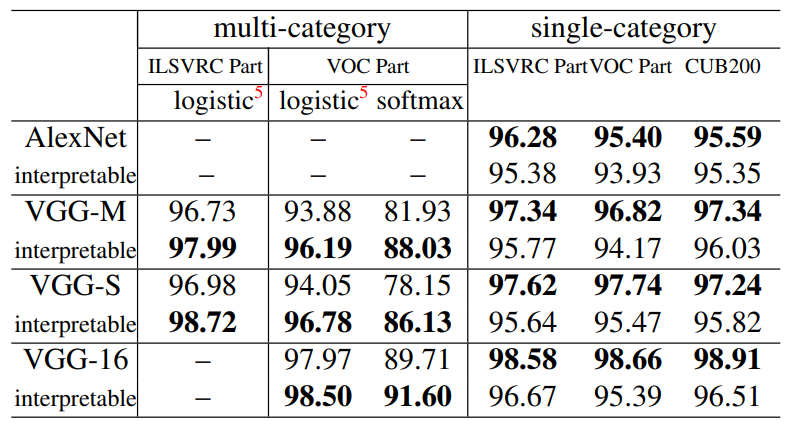
\includegraphics[width=0.6\linewidth]{figures/accuracy.png}
        \caption{Classification accuracy based on different datasets.}
        \label{fig:accuracy}
    \end{figure}
        
    \end{itemize}
\end{frame}

\section{Critical opinion}

\begin{frame}{Pros \& cons}
    \begin{table}[ht]
    \centering
    \begin{tabularx}{\linewidth}{@{}X>{\hsize=.85\hsize}X>{\hsize=.5\hsize}X@{}}
    \toprule
    \textbf{Pros} & \textbf{Cons} \\ \midrule
    Significant gain in metrics & Not useful in many tasks (annotated data needed) \\
    Does not require different data & Higher layers can now just focus on 1 part \\
    Loss function not changed & Lower layers interpretability not assessed \\
    Applicable to several architectures & Filter-category mapping not injective \\
     & Assigned category can change mid-training \\
     & Training process more expensive \& complex \\
    \bottomrule
    \end{tabularx}
    % \caption{Pros and cons}
    % \label{table:pros_cons}
    \end{table}
\end{frame}

\begin{frame}{What would I do now?}
    There are \textbf{two} main \textbf{levels} at which new \textbf{research lines} could be proposed:
    \begin{itemize}
        \item \textbf{Practical} level:
        \begin{itemize}
            \item \textbf{Design} new \textbf{filters} to describe \textbf{discriminative textures} of a category (\textit{lower conv. layers assessed}) % thought for lower conv. layers
            \item \textbf{Design} new \textbf{filters} for object parts shared by multiple categories (\textit{higher model flexibility}) % in order to achieve a higher model flexibility.
            \item \textbf{Design} a \textbf{loss} which regularizes the \textbf{number of part} to \textbf{focus} on (\textit{instead of focusing on a single part per object})
        \end{itemize}
        \item \textbf{Conceptual} level:
        \begin{itemize}
            \item \textbf{Assess} the \textbf{relevance} of individual \textbf{neurons} to the \textbf{decision making} (\textit{interpretability just assessed in terms of capturing useful visual patterns})
        \end{itemize}
    \end{itemize}
\end{frame}

\end{document}